\chapter{2021}
\section*{一、 选择题(本大题共 15 小题,每小题 2 分,共 30 分)}

1 设 \(N\) 是描述问题规模的非负整数,下列程序段的时间复杂度是 (   )。

static int fun(int N) \{

if (N == 1) return 0 ;

return 1 + fun(N/2);

\}

A. \(O\left( {\log N}\right)\) B. \(O\left( N\right)\) C. \(\left( {N\log N}\right)\) D. \(O\left( {N}^{2}\right)\)

2 一些随机产生的数采用线性链表存储, 在下面这些排序方法中, (   )的时间复杂度是最小的。

A. 插入排序 B. 快速排序 C. 堆排序 D. 归并排序

3 一个栈的输入序列为 \(a,b,c,d,e\) ,则下列序列中不可能是栈的输出序列的是 (   )。

A. \({b c d a e}\) B. \({e d a c b}\) C. \({b c a d e}\) D. \({a e d c b}\)

4 实现一个队列需要(   )个栈。

A. 1 B. 2 C. 3 D. 4

5 下面(   )是一颗满二叉树的结点个数。

A. 8 B. 13 C. 14 D. 15

6 若 \(\mathrm{X}\) 是二叉中序线索树中一个有左孩子的结点,且 \(\mathrm{X}\) 不为根, 则 \(\mathrm{X}\) 的前驱为(   )。

A. \(\mathrm{X}\) 的双亲 \hspace{2em} B. X 的右子树中最左的结点

C. \(\mathrm{X}\) 的左子树中最右的结点 D. \(\mathrm{X}\) 的左子树中最右的结点

7 下列序列中, 哪一个是堆 (   )

A.75,65,30,15,25,45,20,10

B.75,65,45,10,30,25,20,15

C.75,45,65,30,15,25,20,15

D.75,45,65,10,25,30,20,15

8 一棵 Huffman 树共有 203 个结点, 对其 Huffman 编码, 共能得到(   )个不同的码字。

A. 100 B. 102 C. 200 D. 203

9 下面说法错误的是(   )。

A. 一个有 n 个顶点和 n 条边的无向图一定是有环的。

B. 建立十字链表的时间复杂度和建立邻接表是相同的。

C. 邻接表只能用于有向图的存储,邻接矩阵对于有向图和无向图的存储都适用。

D. 在某些图的应用问题中, 如果需要找到表示同一条边的两个结点, 那么采用邻接多重表比邻接表作为储存结构更为适宜。

10 图的广度优先遍历算法中使用队列作为其辅助数据结构, 那么在算法执行过程中每个顶点进队次数最多为(   )。

A. 1 B. 2 C. 3 D. 4

11 设一个有向图 \(G = \left( {V,E}\right)\) ,其中

\(V = \left\{  {{v}_{1},{v}_{2},{v}_{3},{v}_{4},{v}_{5},{v}_{6}}\right\}\)

\(E = \left\{  { < {v}_{1},{v}_{2} > , < {v}_{2},{v}_{3} > , < {v}_{3},{v}_{6} > , < {v}_{4},{v}_{2} > , < {v}_{4},{v}_{5} > , < {v}_{5},{v}_{6} > }\right\}\)

不属于该图的拓扑排序有序序列是(   )。

A. \({v}_{1}{v}_{2}{v}_{3}{v}_{4}{v}_{5}{v}_{6}\) B. \({v}_{1}{v}_{4}{v}_{2}{v}_{3}{v}_{5}{v}_{6}\)

C. \({v}_{4}{v}_{5}{v}_{1}{v}_{2}{v}_{3}{v}_{6}\) D. \({v}_{4}{v}_{1}{v}_{2}{v}_{3}{v}_{5}{v}_{6}\)

12 判断一个有向图是否存在回路, 除可利用拓扑排序方法外, 还可以用 (   )。

A. 求关键路径的方法 B. 求最短路径的方法

C. 广度优先遍历的方法 D. 深度优先遍历的方法

13 设有一个二叉排序树 (二叉查找树), 其结点上存储有数字 1 到 100 。现在需要查找数字 55 ,下面(   )序列不可能是查找过程中访问过的结点序列。

A. \(\{ {10},{75},{64},{43},{60},{57},{55}\}\) B. \(\{ {90},{12},{68},{34},{62},{45},{55}\}\)

C. \(\{ 9,{85},{47},{68},{43},{57},{55}\}\) D. \(\{ {79},{14},{72},{56},{16},{53},{55}\}\)

14 在顺序表 \(\{ 2\) 、5、7、10、14、15、18、23、35、41、 \({52}\}\) 中, 用二分法查找关键码 12 需做(   )次关键码比较。

A. 2 B. 3 C. 5 D. 4

15 一颗 3 阶 B-树中有 2047 个关键字, 包括叶结点层, 该树的最大深度为 (   )。

A. 11 B. 12 C. 13 D. 14

\section*{二、填空题(本大题共 10 小题,每小题 3 分,共 30 分)}

16 一颗深度为 \(k\) 的平衡二叉树,其每个非终端结点的平衡因子均为 0 ,则该树共有(   )个结点。

17 设 \( Q \) 表示一个包含十六个元素的队列，\( S \) 为一个空栈。  
Head(Q) 返回队列 \( Q \) 的队头元素，但不将其从队列中移除；  
Top(S) 返回栈 \( S \) 的栈顶元素，但不将其从栈中移除。  

考虑如下算法：
\begin{lstlisting}[language=C, basicstyle=\ttfamily]
while Q != NULL
    if S == NULL 或 Top(S) <= Head(Q)
        x := Dequeue(Q);
        Push(S, x);
    else
        x := Pop(S);
        Enqueue(Q, x);
    end
end
\end{lstlisting}

该算法中，while 循环的最大可能执行次数是（   ）。

18 对于模式串“aabaac”,给出其 next 数组:(   )。

19 现有按中序遍历二叉树的结果为 \({abc}\) ,有 (   ) 种不同形态的二叉树可以得到这一遍历结果。

20 设一棵二叉树有 20 个叶子结点, 则在该树中有 2 个孩子的结点个数为(   )。

21 设 \(\mathrm{G}\) 是一个非连通无向图,有 10 条边,则该图的顶点数至少有(   )个。

22 顺序查找 3 个元素的顺序表, 若查找第 1 、第 2 和第 3 个元素的查找概率分布是 \(1/2\) 、 \(1/3\) 和 \(1/6\) ,则查找任一元素的平均查找长度为 (   )。

23 散列函数有一个共同的性质, 即函数值应当以 (   ) 取其值域的每个值。(请在最大概率、最小概率、平均概率、同等概率这些术语中选择正确的进行填空)

24 假设某算法在输入规模为 \(n\) 时的计算时间为 \(\mathrm{T}\left( n\right)  = {n}^{2}\) 。在某台计算机上实现并完成该算法的时间为 \(t\) 秒。现有另一台计算机, 其运行速度为第一台计算机的 64 倍, 那么在这台计算机上用同一算法在 \(t\) 秒内能解输入规模 (   ) 的问题。

25 表达式 \(a \times  b - c - d\$ e\$ f - g - h \times  i\) 中,运算符的优先级由高到低依次为一,×,\$,均右结合,则相应的后缀式是(   )。

\section*{三、综合应用题 (本大题共 7 小题, 共 60 分)}

26 (10分) 假设称正读和反读都相同的字符序列为“回文”,例如,'abba'和'abcba'是回文,'abcde'和'ababab'则不是回文。下面代码判别读入的一个以‘@’为结束符的字符序列是否是“回文”。请给出缺失的 5 行代码。

Status SymmetryString(char* p)

\{



Queue q;

if(!InitQueue(q)) return 0;

Stack s;

InitStack(s);

ElemType e1, e2;

while(\_\_\_\_\_(1)\_\_\_\_\_)\{

\hspace*{4em} Push(s,*p);

\hspace*{4em} EnQueue(q,*p);

\hspace*{7em} ( 2 )\_\_\_\_\_

\}

while(!StackEmpty(s))\{

\hspace*{8em} (3)

\hspace*{4em} (4)

注:所有答案必须写在答题纸上,试卷上作答无效！ 第 5 页/共 9 页

\hspace*{2em} if(\_\_\_\_\_(5)\_\_\_\_\_) return FALSE;

\hspace*{1em} \}

\hspace*{1em} return OK;

\}

27.(5 分)阅读下面代码:

\begin{lstlisting}[language=C, basicstyle=\ttfamily]
int count = 0;
int N = a.length;
sort(a);
for(int i = 0;i < N;i++) {
    for(int j = i + 1;j < N;j++) {
        if(BinarySearch(a, a[i]+a[j])) count++;
    }
}
\end{lstlisting}


假设当 \(\mathrm{N} = {3500}\) ,上述代码运行 1 秒。那么,当 \(\mathrm{N} = {35000}\) 时,

该代码的运行时间最接近下面那个时间？请给出简单的分析过程。

A.10 seconds B. 20 seconds D. 2 minutes

E. 1 hour F. 2 hours
\vspace{10em}

\newpage
28(8 分)将关键字序列 \(\{ {23},{14},9,6,{30},{12},{18}\}\) 散列存储到散列表中, 散列表的存储空间是一个下标从 0 开始的一维数组, 散列函数为 \(\mathrm{H}\left( \mathrm{{Key}}\right)  = \mathrm{{Key}}\mathrm{{MOD}}7\) ,处理冲突采用线性探测法,要求装填(载)因子为 0.7 。

请画出所构造的散列表。
\vspace{10em}

29 (12 分) 已知一棵二叉树的先序序列: ABDGJEHCFIKL, 中序序列: DJGBEHACKILF。

(1)画出此二叉树的形态。

(2)画出此二叉树的后序线索树。

(3)采用孩子兄弟表示法来存储该二叉树,请画出此二叉树的存储结构。

(4)画出与此二叉树对应的森林。
\vspace{10em}

\newpage
30 (8分) 考虑下列36个字符 (symbol) 的序列: FC F C E C A C

BDEDFEABFBAFFCDCBEDFFFCCDEEF 下面表 30-1 给出了为上述字符序列编码的四种变长编码方式, 即 CODE1、CODE2、CODE3、CODE4; 表 30-2 给出了编码特点, 即 \(\mathrm{A}\text{ 、 }\mathrm{\;B}\text{ 、 }\mathrm{C}\text{ 、 }\mathrm{D}\) ,请给出这 4 种编码方式所具有的编码特点。(填写该编码方式具有的编码特点编号即可,不用给出具体分析过程) 

表 30-1:

\begin{center}
\begin{tabular}{|c|c|c|c|c|c|}
\hline
symbol & frequency & CODE1 & CODE2 & CODE3 & CODE4 \\
\cline{1-6}
A & 3 & 011 & 011 & 1110 & 100 \\
\cline{1-6}
B & 4 & 010 & 010 & 1111 & 101 \\
\cline{1-6}
C & 8 & 00 & 00 & 00 & 01 \\
\cline{1-6}
D & 5 & 110 & 101 & 110 & 110 \\
\cline{1-6}
E & 6 & 001 & 100 & 10 & 111 \\
\cline{1-6}
F & 10 & 10 & 11 & 01 & 00 \\
\cline{1-6}
\hline
\end{tabular}
\end{center}

表 30-2: A. 前缀编码 B. Huffman 编码(能够由 Huffman 算法生成) C. 最优前缀编

CODE1:\_\_\_\_\_ CODE2:\_\_\_\_\_ CODE3 :\_\_\_\_\_ CODE4 :\_\_\_\_\_
\vspace{10em}

31(7 分)图 \(G\) 的邻接矩阵如右边所示:

\begin{center}
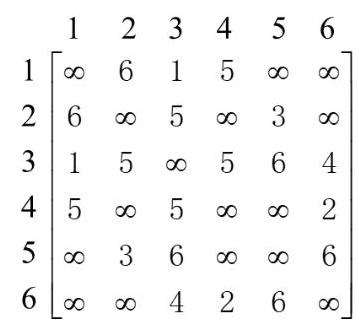
\includegraphics[width=0.3\textwidth]{images/2021/comprehensive_31.jpg}
\end{center}
\hspace*{3em} 

(1)求从顶点 1 出发的广度优先搜索序列；

(2)根据 prim 算法,求图 \(G\) 从顶点 1 出发的最小生成树, 要求表示出其每一步生成过程。
\vspace{10em}

\newpage
32 (10 分) 表 32-1 中,第 0 行是待排序序列的原始输入(12 2 16 30 28 10 16*20 6 18); 其他各行是 5 种排序算法得到的某个中间步骤的内容。表 32-2 列出了 6 种排序算法。请按行序直接给出每行对应排序算法的编号。每个编号只使用一次。

表 32- 排序算法 序列

\begin{center}
\begin{tabular}{|c|c|c|c|c|c|c|c|c|c|c|}
\hline
第 0 行 & 原始输入 & 12 & 2 & 16 & 30 & 28 & 10 & 16* & 20 & 6 \\
\cline{1-11}
算法 & \phantom{X} & 2 & 12 & 16 & 30 & 28 & 10 & 16* & 20 & 6 \\
\cline{1-11}
算法 & \phantom{X} & 6 & 2 & 10 & 12 & 28 & 30 & 16* & 20 & 16 \\
\cline{1-11}
\hline
\end{tabular}
\end{center}

\begin{center}
\begin{tabular}{|c|c|c|c|c|c|c|c|c|c|c|}
\hline
算 法 & \phantom{X} & 2 & 12 & 16 & 30 & 10 & 28 & 16* & 20 & 6 \\
\cline{1-11}
算法 & \phantom{X} & 10 & 2 & 16 & 6 & 18 & 12 & 16* & 20 & 30 \\
\cline{1-11}
算法 & \phantom{X} & 2 & 12 & 16 & 28 & 10 & 16* & 20 & 6 & 18 \\
\cline{1-11}
\hline
\end{tabular}
\end{center}

表 32-2:

\begin{center}
\begin{tabular}{|c|c|}
\hline
排序算法 编号 & 排序算法名称 \\
\cline{1-2}
A & 希尔排序(增量 为 \(5,2,1)\) \\
\cline{1-2}
B & 快速排序 \\
\cline{1-2}
C & 直接选择排序 \\
\cline{1-2}
\hline
\end{tabular}
\end{center}

\begin{center}
\begin{tabular}{|c|c|}
\hline
排序算法 编号 & 排序算法名称 \\
\cline{1-2}
D & 二路归并排序 \\
\cline{1-2}
E & 直接插入排序 \\
\cline{1-2}
F & 冒泡排序 \\
\cline{1-2}
\hline
\end{tabular}
\end{center}
\vspace{10em}

\section*{四、算法分析与设计题(本大题共 2 小题, 每小题 15 分, 共 30 分)}

33 如果一个序列是一个先单调递增后单调递减的序列, 那么它称为双调序列。设计一个尽可能高效的算法,找到由 \(\mathrm{N}\) 个数组成的一个双调序列中最大的关键值。要求:

(1)描述算法的基本设计思想；

(2)根据设计思想,采用 \(\mathrm{C}\) 或 \(\mathrm{C} +  +\) 语言描述算法,关键之处给出注释;

(3)说明你所设计的算法的时间复杂度和空间复杂度。
\vspace{15em}

34 设有一个正整数序列组成的有序单链表 (按递增有序, 且允许有相等的整数存在), 请设计一个用最小的时间和最小空间的算法实现下列功能:(a) 确定在序列中比正整数 \(x\) 大的数有几个 (相同的数只计算一次,如序列 \(\{ 3\text{ 、 }5\text{ 、 }6\text{ 、 }6\text{ 、 }8\text{ 、 }{10}\text{ 、 }{11}\text{ 、 }{13}\text{ 、 }{13}\) 、 \({16}\text{ 、 }{17}\text{ 、 }{20}\text{ 、 }{20}\}\) 中比 10 大的数有 5 个); (b) 将单链表中比正整数 \(x\) 小的数按递减次序排列；(c) 将正整数比 \(x\) 大的偶数从单链表中删除。要求:

(1)描述算法的基本设计思想；

(2)根据设计思想,采用 \(\mathrm{C}\) 或 \(\mathrm{C} +  +\) 语言描述算法,给出注释；

(3)说明你所设计的算法的时间复杂度和空间复杂度。



提示: 节点定义供参考 提示: 算法定义形式供参考

\begin{lstlisting}[language=C, basicstyle=\ttfamily]
typedef struct node {
    int data;
    struct node *next;
}LNode,*LinkList;
\end{lstlisting}

\begin{lstlisting}[language=C, basicstyle=\ttfamily]
void FunctionExam(LinkList L1, int x) 
{
    ......
}
\end{lstlisting}


